\section{Performance comparison} 
\label{sec:performance_comparison}

\begin{figure}
	\centering
	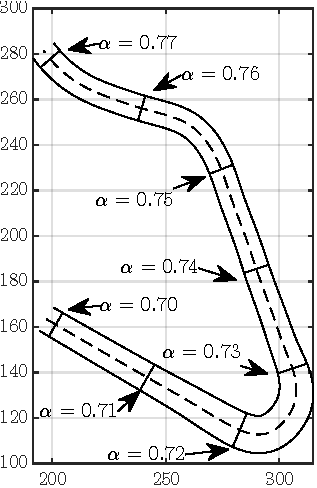
\includegraphics{Fig/track.pdf}
	\caption{Sector of the Catalunya circuit considered in the analysis, corresponding to the curvilinear abscissa interval $\left[0.70, 0.77\right]$. Checkpoints are indicated by labels and are uniformly spaced by $\De\al=0.01$. This sector includes two distinct corners: a low-speed turn from $\al = 0.72$ to $\al = 0.73$, and a high-speed turn from $\al = 0.75$ to $\al = 0.76$, allowing for the evaluation of vehicle behavior across different dynamic scenarios.}
	\label{fig:track}
\end{figure}

\subsection{Open loop parameters sensitivity}
\label{sec:ol_param_sensitivity}
In this section, we explore the open-loop approach to gain deeper insight into the influence of key parameters on the results. For this analysis, we consider optimizations in which only the track limit constraint is robustified. This choice is motivated by the fact that the effects of the track limit constraint are more visually evident compared to those of the friction limit constraint, thereby facilitating a more immediate understanding of their impact. 

The first parameter analyzed is the factor $\ga^\textrm{TLC}$, which multiplies the standard deviation of the constraint, $\sigma^\textrm{TLC}$, to determine the total back-off term $\be^\textrm{TLC}$. This parameter directly influences the probability of satisfying the track limit constraint: higher values of $\ga^\textrm{TLC}$ correspond to more conservative (i.e., robust) behavior. Specifically, $\ga^\textrm{TLC} = 0$ yields a satisfaction probability of 50\%, while $\ga^\textrm{TLC} = 3$ corresponds to 99\%. For the purposes of this analysis, we examine the effect of varying $\ga^\textrm{TLC}$ within this range. 

The second parameter examined is the initial value of the covariance matrix, $\bP_0$. In addition to the baseline value $\bar{\bP}_0$, two alternative values are considered: $\bP_0 = 4\bar{\bP}_0$ and $\bP_0 = \frac{1}{4}\bar{\bP}_0$. These correspond, respectively, to doubling and halving the initial uncertainty associated with the state vector.

\begin{figure}
	\centering
	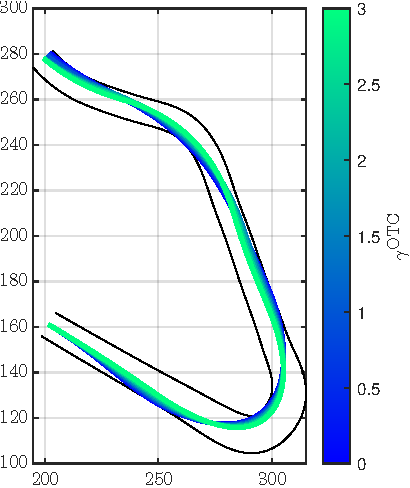
\includegraphics{Fig/gamma_sensitivity.pdf}
	\hfill
	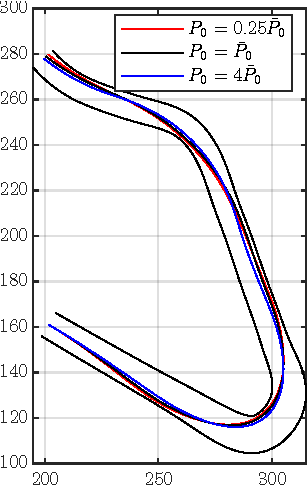
\includegraphics{Fig/Pzero_sensitivity.pdf}
	\caption{Effect of $\ga^\textrm{TLC}$ (left panel) and $P_0$ (right panel) on optimal trajectory. The parameter $\ga^\textrm{TLC}$ span in the range $\left[0,3\right]$ corresponding to a probability to meet the track limit constraint of 50\% and 99\%, respectively. In the left panel, in addition to the baseline value $\bar{\bP}_0$ (black line), two alternative values are considered: $\bP_0 = 4\bar{\bP}_0$ (blue line) and $\bP_0 = \frac{1}{4}\bar{\bP}_0$ (red line). These correspond, respectively, to doubling and halving the initial uncertainty associated with the state vector.}
	\label{fig:ol_sensitivities}
\end{figure}

\subsection{Robustified constraints comparison}
It is of interest to analyze how a robustified constraint---or a combination of the two described in Sections~\ref{sec:FLC} and~\ref{sec:TLC}---influences the driving style. This analysis compares the not-robust trajectory, obtained without robustified constraints, with those resulting from a robustified track limit constraint (denoted as TLC), a robustified friction limit constraint (denoted as FLC), and a scenario where both constraints are robustified (denoted as TLC+FLC). All the optimization are obtained with the open-loop method described in Section~\ref{sec:open_loop_planning}, setting $H=4$, and $\ga^\textrm{TLC}=\ga^\textrm{FLC}=1.28$, corresponding to a 90\% probability of meeting both constraints. 

Figure~\ref{fig:ol_telemetries} presents the variation of four signals with respect to the not-robust trajectory, for the three previously mentioned cases. The panels display the longitudinal speed $u$ (first panel), wheel steering angle $\de$ (second panel), total longitudinal force $F_x$ (third panel), and lateral deviation of the center of mass from the track centerline $e$ (fourth panel). Except for the $u$ panel, each plot includes dashed black lines that indicate the sign of the reference signal-whether it is positive, negative, or numerically zero. These sign indicators are represented as three distinct levels---high, zero, and low---corresponding to positive, zero, and negative values of the reference signal, respectively. The levels are scaled appropriately in each plot to ensure clarity of visualization.

\begin{figure}
	\centering
	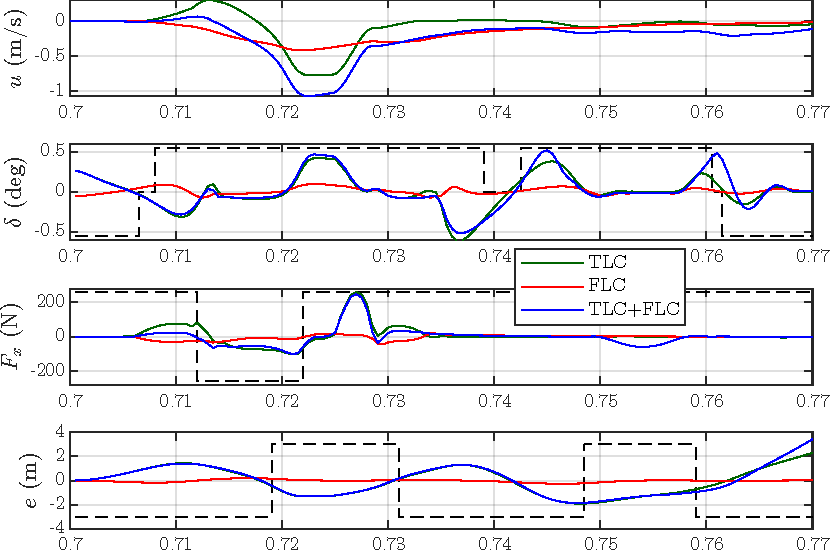
\includegraphics{Fig/ol_telemetries.pdf}
	\caption{Variation of four signals w.r.t. the not-robust trajectory for the three configurations TLC (green line), FLC (red line) and TLC+FLC (blue line). The panels display the longitudinal speed $u$ (first panel), wheel steering angle $\de$ (second panel), total longitudinal force $F_x$ (third panel), and lateral deviation of the center of mass from the track centerline $e$ (fourth panel), over the curvilinear abscissa $\al$. The dashed lines in the last three panels indicate the sign of the reference signal, allowing one to determine whether a positive variation with respect to the baseline corresponds to an increase or a decrease in the absolute value. This distinction is particularly important for quantities that depend on the direction of the turn, such as the wheel steering angle $\de$ and the lateral deviation $e$, while in the case of $F_x$, it indicates whether the vehicle is accelerating or braking.}
	\label{fig:ol_telemetries}
\end{figure}

From the first panel, it can be observed that all configurations maintain a lower mean value of the longitudinal speed compared to the reference trajectory, resulting in an increased sector time. The two configurations incorporating the robustified track limit constraint exhibit, as expected, a significantly altered CoM trajectory. This behavior explains the higher longitudinal speed observed around $\al = 0.71$, which is followed by a sharp reduction. 

The second and fourth panels clearly show that the configurations with the robustified track limit constraint tend to follow a path closer to the centerline. In particular, for most of the sector, the variation in lateral displacement and the lateral displacement $e$ itself exhibit opposite signs, indicating a corrective behavior of the steering angle $\de$ that pulls the vehicle toward the centerline.

It can be interesting to notice that, in the third panel, only the configuration with both the constraints robustified needs to reduce the longitudinal force during the high speed turn, in the curvilinear abscissa interval $\al\in\left[0.75, 0.76\right]$, to meet both the constraints. 
The vehicle constrained by the track limit condition is forced to follow a wider trajectory, which entails greater lateral acceleration and, consequently, a higher lateral force demand---resulting in increased tire utilization. Due to the limitations imposed by the robust friction limit constraint, it is necessary to reduce the available accelerating force.

\begin{figure}
	\centering
	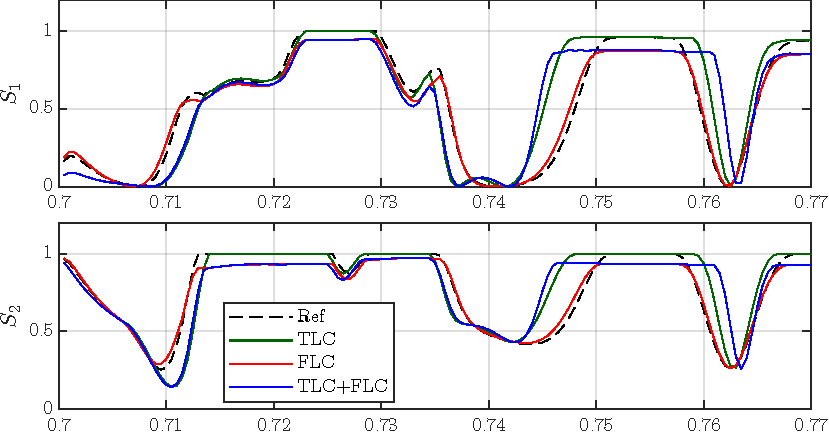
\includegraphics{Fig/ol_saturation.pdf}
	\caption{Tyre usage for front axle (first panel) and rear axle (second panel) over curvilinear abscissa $\al$. The plotted lines represent the quantity $\left[ \left( \frac{X_j(\bx,\bu)}{\mu_{x,j}} \right)^2+ \left( \frac{Y_j(\bx,\bu)}{\mu_{y,j}}\right)^2\right]\frac{1}{Z_j^2(\bx,\bu)}$, where $j=1$ denotes the front axle and $j=2$ the rear axle. The dashed black line corresponds to the reference (not-robust) configuration, while the green, red, and blue lines represent the robust configurations TLC, FLC, and TLC+FLC, respectively.}
	\label{fig:ol_saturation}
\end{figure}

\subsection{Simulations with noise realization}
This analysis aims to provide empirical validation of the robust trajectories obtained using the methods proposed in this work. For conciseness, the comparison is limited to a nominal trajectory and a trajectory computed using the closed-loop method with only the track limit constraint robustified.
An LQR controller, designed according to the procedure outlined in Section~\ref{sec:LQR}, is implemented along the not-robust trajectory. In contrast, the robust trajectory is tracked using the controller directly obtained from the optimization process.

\begin{figure}
	\centering
	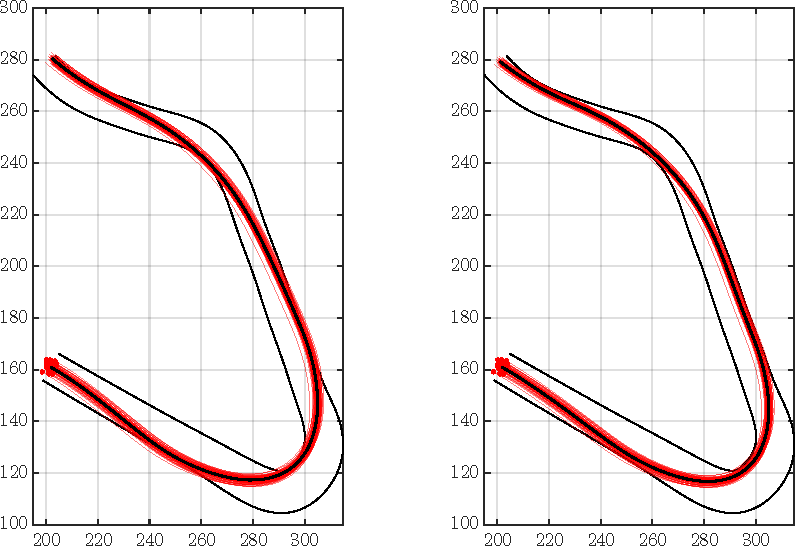
\includegraphics{Fig/olcl_traj_strings.pdf}
	\caption{Simulations with random initial conditions and Gaussian noise realizations. In the left panel, the reference trajectory is the non-robust one, tracked using an LQR controller designed around it. In the right panel, the reference is a robust trajectory obtained using the closed-loop optimization method, and it is tracked using the corresponding optimized controller produced by the same method.}
	\label{fig:traj_strings}
\end{figure}